\documentclass[letterpaper,10pt,conference]{ieeeconf}
\IEEEoverridecommandlockouts
\overrideIEEEmargins
\usepackage{amsmath,amssymb,graphicx,url}
\title{ROS Lab 2: Two-Drone Coordinate Transforms and Cloud Validation}
\author{Course Laboratory Report}
\begin{document}
\maketitle

\begin{abstract}
This report implements and tests the MIT VNAV Lab 2 two-drone transformation exercise. The course's ROS 1 Noetic package was built in an Ubuntu 20.04 environment on the provided cloud host, then exercised with turtlesim, static and dynamic tf, RViz, and five visualization markers. Thirty live relative-pose samples satisfied the derived plane and ellipse equations to numerical precision. An equivalent ROS 2 Humble package was also built and tested on the host. The second vehicle follows a parabolic arc in the world $x$--$z$ plane but an ellipse in the first vehicle's body frame.
\end{abstract}

\section{Scope and Environment}
The course slides prescribe Ubuntu 20.04 with ROS Noetic, starting \texttt{roscore}, verifying node communication with turtlesim, and completing the MIT tf and mathematical exercises \cite{course,mit}. The ROS 1 source is based on the MIT-SPARK \texttt{VNAV2023} tag \cite{code}; the separately supplied cloud implementation is based on the repository's ROS 2 main branch \cite{code2}. Their message and build APIs differ, but both encode the same world poses and relative-pose queries. This report uses the IEEE Robotics and Automation Society's \texttt{ieeeconf} template \cite{template} as an ICRA-style course-report layout.

The ROS 1 reproduction commands are in \texttt{lab2/RUN.md}; on Ubuntu 20.04 they require Noetic \cite{noetic}. The cloud host itself ran Ubuntu 22.04.3 with ROS 2 Humble. To execute the course version, we created an Ubuntu 20.04 Focal root filesystem on that host, installed ROS Noetic and the required build tools there, and built the package with \texttt{catkin build} (also checked with \texttt{catkin\_make}). The supplementary native-host path in \texttt{lab2/ros2\_ws/RUN.md} uses \texttt{colcon build} and \texttt{ros2 launch}. Both turtlesim controllers publish \texttt{geometry\_msgs/Twist} at 20 Hz with linear $x=1$ and angular $z=1$. The two-drone scene visualizes idealized poses; it does not simulate flight dynamics or command quadrotor motors.

\section{ROS Graph and Implementation}
\subsection{Static and Dynamic Graphs}
With \texttt{static:=true}, the course's \texttt{two\_drones.launch} starts \texttt{/av1broadcaster} and \texttt{/av2broadcaster}, each publishing a fixed transform from \texttt{world} on \texttt{/tf\_static}. It also starts \texttt{/plots\_publisher\_node}, which subscribes to tf and publishes mesh and trail markers on \texttt{/visuals}, and \texttt{/rviz}, which subscribes to both. The ROS 2 cloud launch has the same graph except that its visualizer is \texttt{/rviz2\_node}. AV1 starts at $(1,0,0)$ and AV2 at $(0,0,1)$. Ignoring tf listener helpers, these are the four primary launch nodes. The meshes originate from \texttt{/visuals}, not from the static broadcasters. Figure~\ref{fig:tfgraph} summarizes the observed frame and marker relationships.

\begin{figure}[t]
\centering
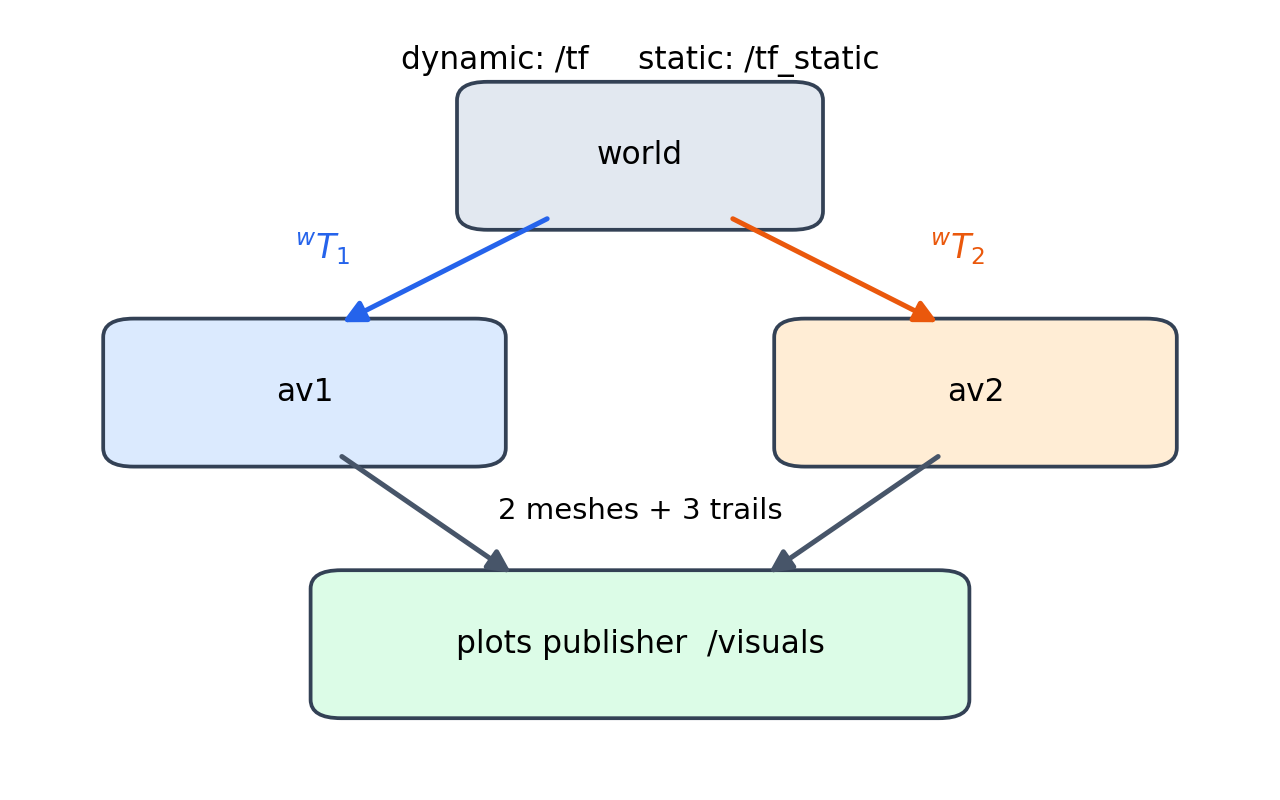
\includegraphics[width=\columnwidth]{tf_graph.png}
\caption{The world-to-drone tf tree and marker flow. The same edges use \texttt{/tf\_static} in the static run and \texttt{/tf} in the dynamic run. The plot node publishes two meshes and three trails on \texttt{/visuals}.}
\label{fig:tfgraph}
\end{figure}

As requested by the 2023 exercise, the ROS 1 static graph can be started manually after \texttt{roscore}, with each command in a separate sourced terminal:
\begin{small}
\begin{verbatim}
rosrun tf2_ros static_transform_publisher \
  1 0 0 0 0 0 1 world av1
rosrun tf2_ros static_transform_publisher \
  0 0 1 0 0 0 1 world av2
rosrun two_drones_pkg plots_publisher_node
rosrun rviz rviz -d $(rospack find \
  two_drones_pkg)/config/default.rviz
\end{verbatim}
\end{small}
Without \texttt{static:=true}, the launch files' \texttt{if} branch excludes the static broadcasters and the \texttt{unless} branch starts \texttt{/frames\_publisher\_node}. That node publishes changing \texttt{world}$\rightarrow$\texttt{av1} and \texttt{world}$\rightarrow$\texttt{av2} poses on \texttt{/tf}. The plot node produces world-frame traces for both vehicles and an AV2-in-AV1 trace. Setting the RViz fixed frame to \texttt{av1} makes AV1 appear stationary.

\subsection{Pose Publication and Lookup}
Let $t$ be seconds since the publisher started. The assignment specifies
\begin{equation}
{}^w\mathbf{o}_1=(\cos t,\sin t,0)^T,\quad
{}^w\mathbf{o}_2=(\sin t,0,\cos 2t)^T.
\label{eq:positions}
\end{equation}
AV1 has zero roll and pitch and yaw $t$, so its $y$ axis is $(-\sin t,\cos t,0)^T$, tangent to its circular path. AV2 retains the world orientation. Both implementations stamp \texttt{TransformStamped} messages with the same ROS time, use \texttt{tf2::Quaternion::setRPY(0,0,t)} for AV1, and broadcast both transforms at 50 Hz. Their plot nodes query the latest transform with \texttt{lookupTransform(ref\_frame,dest\_frame,...)}, which returns the destination pose expressed in the reference frame. The ROS 1 listener constructs its tf buffer first and uses a bounded timeout; the ROS 2 listener catches unavailable-frame exceptions during startup.

\section{Mathematical Derivations}
\subsection{World-Frame Parabola and Relative Pose}
For AV2, $x=\sin t$, $y=0$, and $z=\cos 2t=1-2\sin^2t=1-2x^2$. Because $x\in[-1,1]$, the world path is the arc $z=1-2x^2$ in the $x$--$z$ plane, traversed repeatedly. Figure~\ref{fig:world3d} shows its spatial relation to AV1's circle.

\begin{figure}[t]
\centering
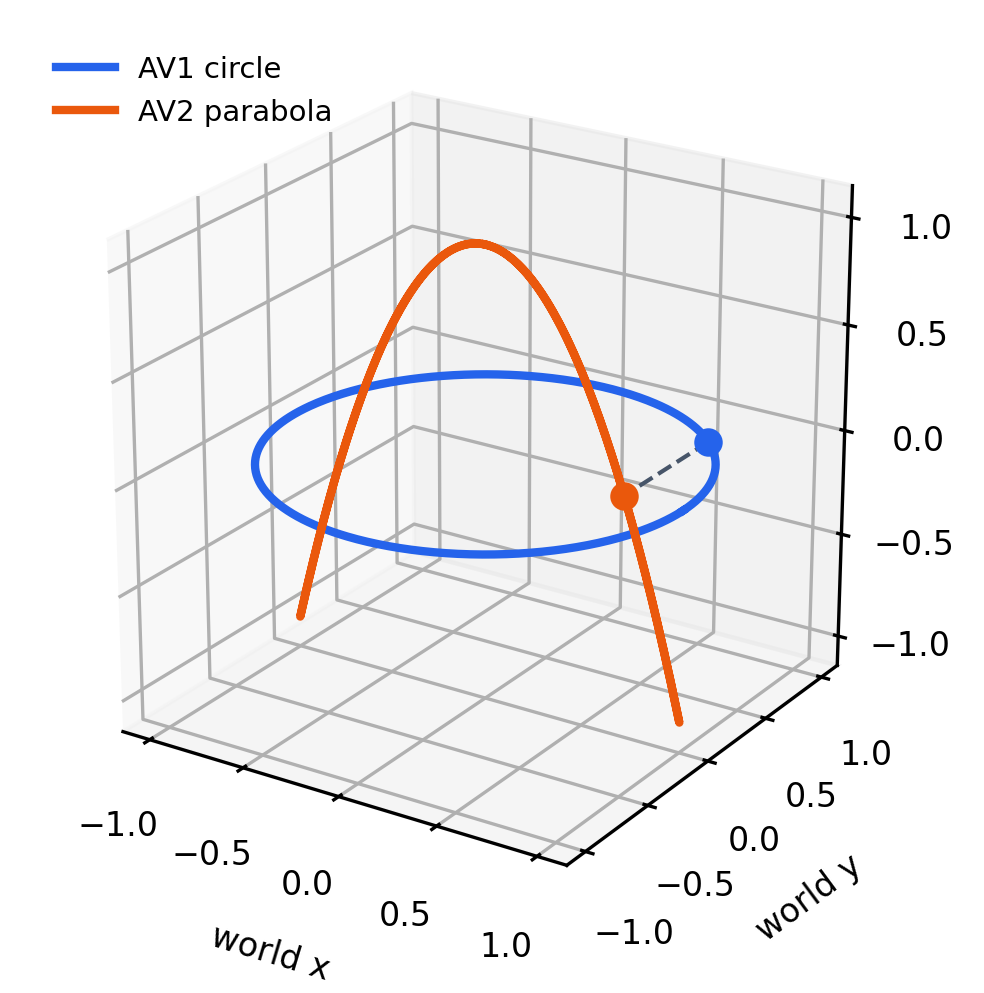
\includegraphics[width=0.97\columnwidth]{world_3d.png}
\caption{Analytical three-dimensional world trajectories. Dots mark both poses at $t=\pi/4$; the dashed segment joins them. This is computed from Eq.~\eqref{eq:positions}, not an RViz screenshot.}
\label{fig:world3d}
\end{figure}

Write $c=\cos t$ and $s=\sin t$. With $^wR_1=R_z(t)$ and $^wR_2=I$, the homogeneous transforms and composition are
\begin{equation}
{}^wT_1=\begin{bmatrix}c&-s&0&c\\s&c&0&s\\0&0&1&0\\0&0&0&1\end{bmatrix},
\end{equation}
\begin{equation}
{}^wT_2=\begin{bmatrix}1&0&0&s\\0&1&0&0\\0&0&1&\cos2t\\0&0&0&1\end{bmatrix}.
\end{equation}
Their composition is
\begin{equation}
{}^1T_2=({}^wT_1)^{-1}{}^wT_2
=\begin{bmatrix}c&s&0&cs-1\\-s&c&0&-s^2\\0&0&1&\cos2t\\0&0&0&1\end{bmatrix}.
\label{eq:relative}
\end{equation}
Consequently, $^1\mathbf{o}_2=(cs-1,-s^2,\cos2t)^T$. The plane relation follows from $-s^2=(\cos2t-1)/2$:
\begin{equation}
\Pi:\quad z_2^1-2y_2^1=1.
\label{eq:plane}
\end{equation}

\subsection{Planar Coordinates and Ellipse}
Choose the center $\mathbf{p}^1=(-1,-1/2,0)^T$, the unit plane axes $\mathbf{e}_x=(1,0,0)^T$ and $\mathbf{e}_y=(0,1,2)^T/\sqrt5$, and normal $\mathbf{e}_z=(0,-2,1)^T/\sqrt5$. The matrix $^1R_p=[\mathbf{e}_x\ \mathbf{e}_y\ \mathbf{e}_z]$ has determinant $+1$, and
\begin{equation}
{}^1T_p=\begin{bmatrix}{}^1R_p&\mathbf{p}^1\\0&1\end{bmatrix},\quad
{}^pT_2=({}^1T_p)^{-1}{}^1T_2.
\end{equation}
Applying the inverse transform to AV2's origin gives
\begin{equation}
{}^p\mathbf{o}_2=\left(\tfrac12\sin2t,\tfrac{\sqrt5}{2}\cos2t,0\right)^T.
\label{eq:ellipseparam}
\end{equation}
Thus $(x_p/(1/2))^2+(y_p/(\sqrt5/2))^2=1$. The semi-axis lengths are $1/2$ and $\sqrt5/2$. Figure~\ref{fig:paths} is generated from these equations, not captured from RViz.

\begin{figure}[t]
\centering
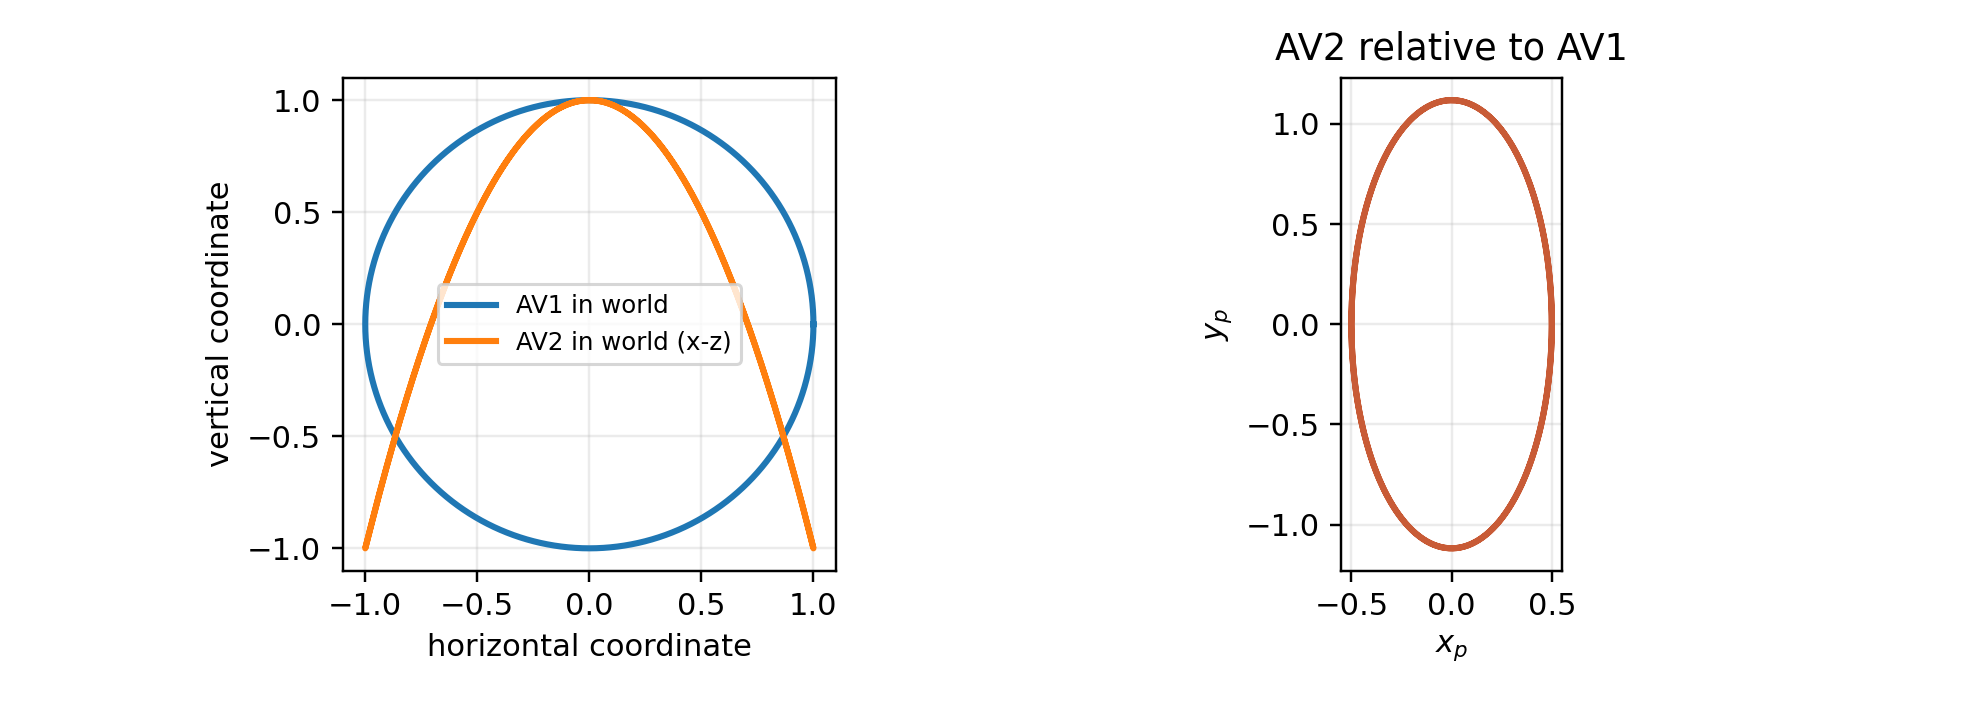
\includegraphics[width=\columnwidth]{trajectories.png}
\caption{Analytical world-frame trajectories (left) and AV2 relative to AV1 in the plane coordinates (right). The two curves on the left use different world-coordinate planes and are shown together only for comparison.}
\label{fig:paths}
\end{figure}

\section{Quaternion Properties}
The course defines $\Omega_1(q)$ and $\Omega_2(q)$ as the matrices for left and right Hamilton multiplication, using scalar-last vectors: $\Omega_1(a)b=a\otimes b=\Omega_2(b)a$. The quaternion norm is multiplicative, $\|a\otimes b\|=\|a\|\|b\|$. If $q$ is unit, both maps preserve the norm of every vector in $\mathbb R^4$. A linear norm-preserving map is orthogonal (by the polarization identity), hence
\begin{equation}
\Omega_i(q)^T\Omega_i(q)=\Omega_i(q)\Omega_i(q)^T=I_4,\quad i=1,2.
\end{equation}
For $e=(0,0,0,1)^T$, the identity quaternion, $\Omega_i(q)e=q$ for either $i$. Orthogonality then gives $\Omega_i(q)^Tq=e$.

Associativity proves the remaining identities without a 16-entry expansion. For arbitrary $x,y,z$, $x\otimes(z\otimes y)=(x\otimes z)\otimes y$ implies $\Omega_1(x)\Omega_2(y)=\Omega_2(y)\Omega_1(x)$. Right multiplication by the conjugate $\bar y=(-y_1,-y_2,-y_3,y_4)^T$ is the transpose of right multiplication by $y$, so $\Omega_2(y)^T=\Omega_2(\bar y)$. Substituting $\bar y$ in the first identity gives $\Omega_1(x)\Omega_2(y)^T=\Omega_2(y)^T\Omega_1(x)$. This argument holds even when $x$ and $y$ are not unit.

\section{Cloud Experiment and Verification}
The Focal environment reported \texttt{ROS\_DISTRO=noetic}. The course package compiled both C++ nodes with \texttt{catkin build -j1}; its summary reported two successful targets and zero failures. A separate \texttt{catkin\_make -j1} build passed. A Noetic \texttt{roscore} served the graph; turtlesim ran under Xvfb. Its pose changed from $(5.5444,5.5444,0)$ at rest to $(5.1156,7.4516,-2.7152)$ after the controller published linear $x=1$ and angular $z=1$ on \texttt{/turtle1/cmd\_vel}. The observed pose velocities were both 1, and the controller exited successfully.

In the Noetic dynamic launch, \texttt{/frames\_publisher\_node} published \texttt{/tf}, while \texttt{/plots\_publisher\_node} published \texttt{/visuals}; RViz subscribed to both. A live verifier collected 30 tf samples and 139 MarkerArray messages, each containing two meshes and three trails. Maximum residuals were $2.22\times10^{-16}$ for the AV2 parabola, $4.44\times10^{-16}$ for Eq.~\eqref{eq:plane}, and $1.78\times10^{-15}$ for the ellipse. Independently fetched latest transforms differed by up to $0.0426$ because their timestamps were asynchronous. The static Noetic launch had two \texttt{/tf\_static} publishers. A second verifier measured the expected AV1 and AV2 translations $(1,0,0)$ and $(0,0,1)$, identity rotations, and five markers.

\begin{figure}[t]
\centering
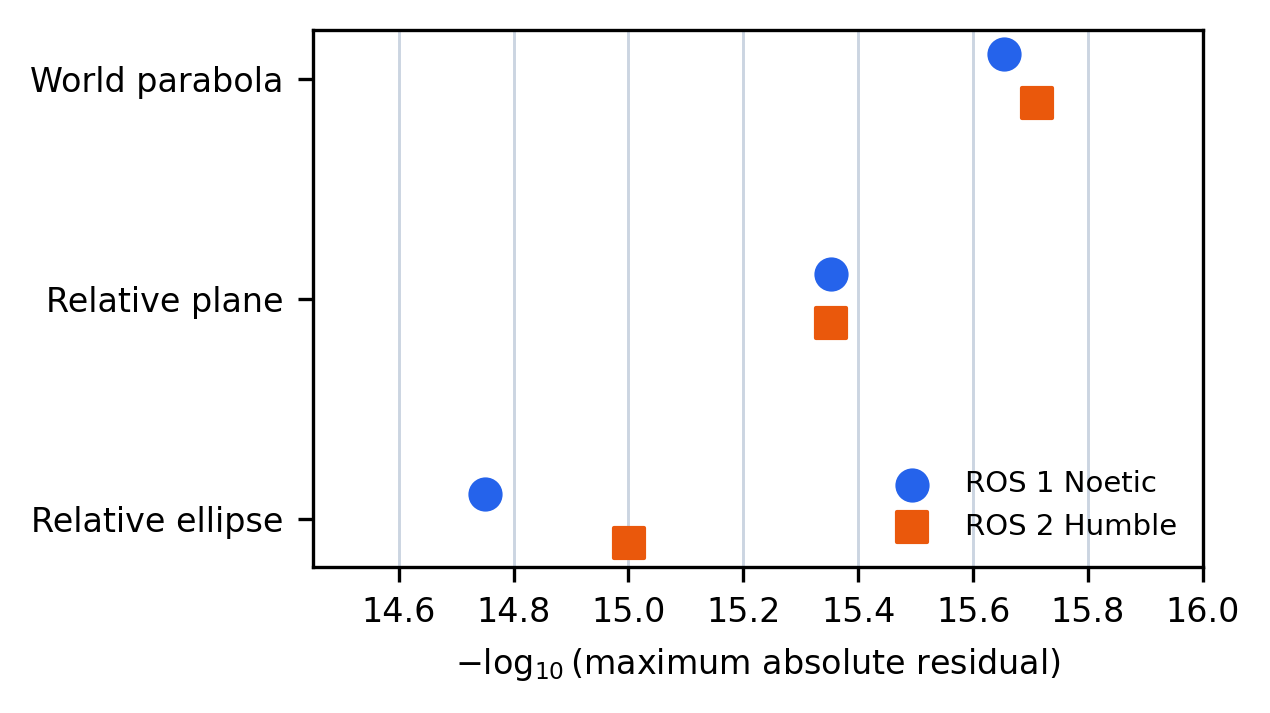
\includegraphics[width=\columnwidth]{precision.png}
\caption{Precision of the live trajectory checks in both ROS versions. Larger values on the horizontal axis mean smaller maximum residuals. Each result was computed from 30 tf samples; marker counts are reported in Table~\ref{tab:checks}.}
\label{fig:precision}
\end{figure}

On the native Ubuntu 22.04 host, the ROS 2 Humble counterpart passed \texttt{colcon build} in 50.9 s. Its dynamic verifier sampled 30 tf transforms and 14 MarkerArrays with five markers each; the plane and ellipse residuals were below $10^{-15}$. Its static graph and turtlesim controller also passed. Table~\ref{tab:checks} summarizes the run coverage, and Fig.~\ref{fig:precision} compares the measured residuals. Local checks confirmed the trajectory identities at 1001 times below $10^{-12}$ residual and quaternion identities on 1000 deterministic samples. Raw cloud logs accompany the deliverables. Analytical plots here come from equations rather than RViz screenshots; the optional rotation-order proof is supplied separately.

\begin{table}[t]
\centering
\caption{Cloud runtime verification}
\label{tab:checks}
\begin{tabular}{lccc}
\hline
System & tf samples & MarkerArrays & Static check \\
\hline
Noetic & 30 & 139 & pass \\
Humble & 30 & 14 & pass \\
\hline
\end{tabular}
\end{table}

\begin{thebibliography}{6}
\bibitem{course} Y. Yang, ``Visual SLAM / Robot Integration: Experiment II,'' course slides, supplied \texttt{Lab2.pdf}.
\bibitem{mit} MIT VNAV, ``Lab 2 Exercises,'' 2023. [Online]. Available: \url{https://vnav.mit.edu/labs_2023/lab2/exercises.html}
\bibitem{code} MIT-SPARK, ``VNAV-labs,'' \texttt{VNAV2023} tag. [Online]. Available: \url{https://github.com/MIT-SPARK/VNAV-labs/tree/VNAV2023/lab2}
\bibitem{code2} MIT-SPARK, ``VNAV-labs,'' ROS 2 main branch. [Online]. Available: \url{https://github.com/MIT-SPARK/VNAV-labs/tree/main/lab2}
\bibitem{template} IEEE Robotics and Automation Society, ``(La)TeX Support for manuscript preparation.'' [Online]. Available: \url{https://ras.papercept.net/conferences/support/tex.php}
\bibitem{noetic} ROS Wiki, ``noetic/Installation/Ubuntu.'' [Online]. Available: \url{https://wiki.ros.org/noetic/Installation/Ubuntu}
\end{thebibliography}
\end{document}
